\documentclass[8pt, xcolor={svgnames}, hyperref={linkcolor=black}]{beamer}
\usepackage[labelfont={color=amethyst,bf}]{caption}
\setbeamercolor{background canvas}{bg=white}
\usetheme[progressbar=frametitle]{metropolis}
\usepackage{appendixnumberbeamer}
\usepackage{url}
\usepackage{booktabs}
\usepackage{braket}
\usepackage[scale=2]{ccicons}
\usepackage{amsfonts} 
\usepackage{amssymb}
\usepackage[english]{babel}
\colorlet{col1}{teal}
\colorlet{col2}{yellow}
\colorlet{col3}{green}
\usepackage{fontawesome}
\usepackage{subcaption}
\usepackage{overpic} 
\usepackage{multicol}
\usepackage{bm}
\usepackage{algorithm}
\usepackage{algpseudocode}
\usepackage{enumitem}

\usepackage[]{pseudo}


\usepackage{tikz}
\usetikzlibrary{positioning,arrows,calc,math,angles,quotes}
\usepackage{blochsphere}

\usetikzlibrary{arrows,automata}
\usetikzlibrary{positioning}
\usetikzlibrary{arrows.meta,
                bending,
                intersections,
                quotes,
                shapes.geometric}

\tikzset{
    state/.style={
           rectangle,
           rounded corners,
           draw=black, very thick,
           minimum height=1em,
           inner sep=2pt,
           text centered,
           },
}


\definecolor{myv}{rgb}{0.36, 0.22, 0.33}
\definecolor{gio}{rgb}{0.45, 0.31, 0.59}
\definecolor{light}{rgb}{0.8, 0.8, 1}
\definecolor{warmblack}{rgb}{0.0, 0.26, 0.26}
\definecolor{brown(web)}{rgb}{0.65, 0.16, 0.16}
\definecolor{cadmiumgreen}{rgb}{0.0, 0.42, 0.24}
\definecolor{darkmidnightblue}{rgb}{0.0, 0.2, 0.4}
\definecolor{brightube}{rgb}{0.82, 0.62, 0.91}

\definecolor{codegreen}{rgb}{0,0.6,0}
\definecolor{codegray}{rgb}{0.5,0.5,0.5}
\definecolor{codepurple}{rgb}{0.58,0,0.82}
\definecolor{backcolour}{rgb}{0.95,0.95,0.92}
\definecolor{amethyst}{rgb}{0.6, 0.33, 0.73}

\definecolor{light-gray}{gray}{0.95}
\newcommand{\code}[1]{\colorbox{light-gray}{\texttt{#1}}}
\newcommand{\equals}{=}

\usepackage[most]{tcolorbox}
\usepackage{xcolor}

%\usepackage[citecolor = green, linkcolor = blue, bookmarks=true, urlcolor=blue,
%colorlinks=true, pagebackref=true]{hyperref}


%\usepackage{xspace}

\title{Real-time quantum error mitigation in training VQAs}
\date{}
\author[Matteo Robbiati, Alejandro Sopena, Andrea Papaluca, Stefano Carrazza]{Matteo Robbiati, Alejandro Sopena, Andrea Papaluca, Stefano Carrazza}
\subtitle{Based on: \href{https://arxiv.org/abs/2311.05680}{\faBook\,\,arXiv:2311.05680}}
\titlegraphic{
\begin{tikzpicture}[overlay, remember picture]

\node[at=(current page.south east), anchor=south east] {%
\includegraphics[width=.18\textwidth]{figures/qibo.png} 

\includegraphics[width=.18\textwidth]{figures/unimi.png} 
\includegraphics[width=.18\textwidth]{figures/cern.png}  
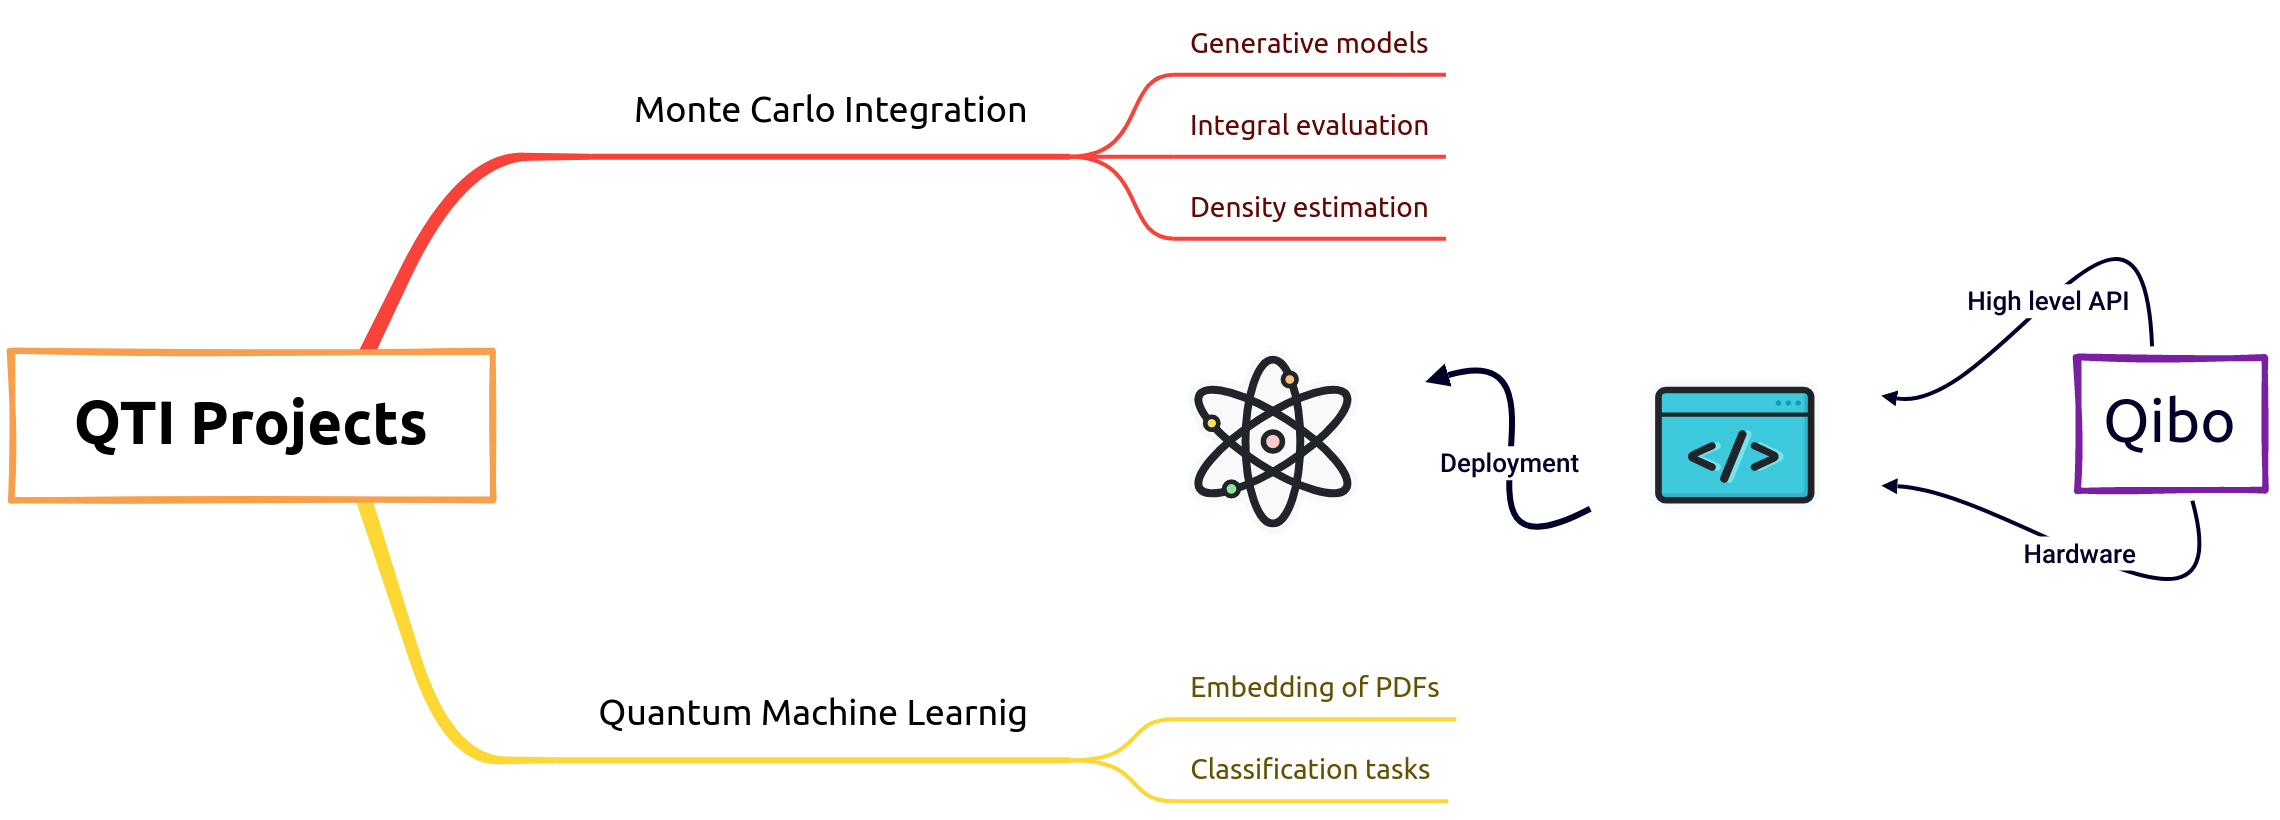
\includegraphics[width=.18\textwidth]{figures/qti.png}  
};
\end{tikzpicture}
}


\begin{document}


\maketitle

\section{Prologue}


\begin{frame}{How did we start? \hfill \href{https://arxiv.org/abs/2109.01051}{\faBook\,\,arXiv:2109.01051}}
\pause
\begin{multicols}{2}
\begin{figure}
\includegraphics[width=0.45\textwidth, height=0.8\textheight]{figures/tii_lab.png}
\caption*{For a 360° tour \href{https://files-prod.tii.ae/360/TII-QRC-Computing-Lab.html}{\texttt{click here!}}}
\end{figure}
\pause
\begin{figure}
\includegraphics[width=0.45\textwidth, height=0.8\textheight]{figures/NIBP_cropped.pdf}
\caption*{Credits to \href{https://arxiv.org/abs/2109.01051}{\faBook\,arXiv:2109.01051}}
\end{figure}
\end{multicols}
\end{frame}

\begin{frame}{How did we start? \hfill \href{https://arxiv.org/abs/2109.01051}{\faBook\,\,arXiv:2109.01051}}
\begin{multicols}{2}
\begin{figure}
\includegraphics[width=0.45\textwidth, height=0.8\textheight]{figures/tii_lab.png}
\caption*{For a 360° tour \href{https://files-prod.tii.ae/360/TII-QRC-Computing-Lab.html}{\texttt{click here!}}}
\end{figure}
\begin{figure}
\includegraphics[width=0.45\textwidth, height=0.8\textheight]{figures/NIBP_1.png}
\caption*{Credits to \href{https://arxiv.org/abs/2109.01051}{\faBook\,arXiv:2109.01051}}
\end{figure}
\end{multicols}
\end{frame}

\begin{frame}{How did we start? \hfill \href{https://arxiv.org/abs/2109.01051}{\faBook\,\,arXiv:2109.01051}}
\begin{multicols}{2}
\begin{figure}
\includegraphics[width=0.45\textwidth, height=0.8\textheight]{figures/tii_lab.png}
\caption*{For a 360° tour \href{https://files-prod.tii.ae/360/TII-QRC-Computing-Lab.html}{\texttt{click here!}}}
\end{figure}
\begin{figure}
\includegraphics[width=0.45\textwidth, height=0.8\textheight]{figures/NIBP_2.png}
\caption*{Credits to \href{https://arxiv.org/abs/2109.01051}{\faBook\,arXiv:2109.01051}}
\end{figure}
\end{multicols}
\end{frame}

\begin{frame}{How did we start? \hfill \href{https://arxiv.org/abs/2109.01051}{\faBook\,\,arXiv:2109.01051}}
\begin{multicols}{2}
\begin{figure}
\includegraphics[width=0.45\textwidth, height=0.8\textheight]{figures/tii_lab.png}
\caption*{For a 360° tour \href{https://files-prod.tii.ae/360/TII-QRC-Computing-Lab.html}{\texttt{click here!}}}
\end{figure}
\begin{figure}
\includegraphics[width=0.45\textwidth, height=0.8\textheight]{figures/NIBP_3.png}
\caption*{Credits to \href{https://arxiv.org/abs/2109.01051}{\faBook\,arXiv:2109.01051}}
\end{figure}
\end{multicols}
\end{frame}

\begin{frame}{How did we start? \hfill \href{https://arxiv.org/abs/2109.01051}{\faBook\,\,arXiv:2109.01051}}
\begin{multicols}{2}
\begin{figure}
\includegraphics[width=0.45\textwidth, height=0.8\textheight]{figures/tii_lab.png}
\caption*{For a 360° tour \href{https://files-prod.tii.ae/360/TII-QRC-Computing-Lab.html}{\texttt{click here!}}}
\end{figure}
\begin{figure}
\includegraphics[width=0.45\textwidth, height=0.8\textheight]{figures/NIBP_cropped.pdf}
\caption*{Credits to \href{https://arxiv.org/abs/2109.01051}{\faBook\,arXiv:2109.01051}}
\end{figure}
\end{multicols}
\begin{picture}(0,0)
    \put(-5,70){
        \includegraphics[width=1\textwidth]{figures/fusion.png}
    }
\end{picture}
\end{frame}

\begin{frame}{Step 1: about noise}
\begin{figure}
\includegraphics[width=1\textwidth]{figures/norm.pdf}
\end{figure}
\end{frame}

\begin{frame}{Step 1: about noise}
\begin{figure}
\includegraphics[width=1\textwidth]{figures/conc.pdf}
\end{figure}
\end{frame}

\begin{frame}{Step 1: about noise}
\begin{figure}
\includegraphics[width=1\textwidth]{figures/corr.pdf}
\end{figure}
\end{frame}

\section{A case study}

\begin{frame}{Step 2: a proper target}
\pause
\begin{tcolorbox}[colback=red!20, title=\faCrosshairs\,\, $N$-dim fit: $y \equals g(\bm{x})$]
We build an $N$ qubits circuit $\mathcal{U}(\bm{x}; \bm{\theta})$:
\begin{figure}
\includegraphics[width=1\textwidth]{figures/circ.pdf}
\end{figure}
\vspace{-0.3cm}
with $x_j$ uploaded twice at layer $\ell$ through the uploading channel $U(x_j; \bm{\theta}_j^{\ell})$.
\end{tcolorbox}
\pause
\begin{tcolorbox}[colback=blue!20, title=\faPaypal\,\, Cost function]
We want a cost function $C$ which suffers of \textbf{cost corruption} and \textbf{concentration}:
$$ C_{\rm mse}(\bm{x}|\bm{\theta}) = \frac{1}{N_{\rm data}}\sum_i^{N_{\rm data}} 
  \bigl[ f(\bm{x}^i,\bm{\theta})_{\mathcal{O}} - g(\bm{x}^i) \bigr]^2 \, $$
$$ \text{with} \qquad 
  f(\bm{x}^i,\bm{\theta})_{\mathcal{O}} = \braket{\psi_0 |\, \mathcal{U}^{\dagger}(\bm{x}^i; \bm{\theta}) \,
  \mathcal{O} \, \mathcal{U}(\bm{x}^i; \bm{\theta})| \psi_0} \qquad \text{and} \qquad 
  \mathcal{O}=\sigma_z^{\otimes N}.$$
\end{tcolorbox}
\end{frame}

\begin{frame}{Step 3: noise model \hfill \href{https://arxiv.org/abs/2007.14384}{\faBook\,\,arXiv:2007.14384}}
We consider local pauli noise and bit-flip readout noise channels.
\pause
\begin{figure}
\includegraphics[width=1\textwidth]{figures/noisy.pdf}
\end{figure}
\pause
In particular:
\begin{itemize}[noitemsep]
\item[\faVolumeUp] $PN$ channel with probs. $-1 < q_x, q_y, q_z < 1$
on each qubit after each layer;
\item[\faRandom] symmetric readout noise $\mathcal{M}$ of single-qubit bit-flip $(BF)$ 
with prob. $(1-q_M)/2$.
\end{itemize}
\pause
The effect of such a noise on our predictor is a cost concentration of the expectation
values around zero:
\pause
$$ |f_{\rm noisy}| < 2 q_M^N q^{2l + 2} \biggl(1-\frac{1}{2^N}\biggr) $$
\end{frame}

\begin{frame}{Can quantum error mitigation help?\hfill \href{https://arxiv.org/abs/2109.01051}{\faBook\,\,arXiv:2109.01051}}
\begin{multicols}{2}
\begin{figure}
    \includegraphics[width=0.45\textwidth]{figures/NIBP_cropped.pdf}
\end{figure}
\pause
\begin{itemize}[noitemsep]
\item[1.] Let's consider $\bm{\theta_1}$ and $\bm{\theta_2}$;
\pause
\item[2.] thus two cost $C(\bm{\theta_1})$, $C(\bm{\theta_2})$;
\pause
\item[3.] noise and QEM affects resolvability;
\pause
\item[4.] let's define a metric: 
\vspace{-0.2cm}
$$ \chi(\bm{\theta_1}, \bm{\theta_2}) = \frac{N_{\rm shots}^{\rm noisy}}{N_{\rm shots}^{\rm mit}}$$
\pause
\vspace{-0.5cm}
\item[5.] we like it if $\chi \geq 1$!
\pause
\item[6.] for Clifford Data Regression $\chi=1$ under Global depolarizing noise given any $\bm{\theta_1}$ and $\bm{\theta_2}$.
\end{itemize}
\pause
\small
\begin{tcolorbox}[colback=blue!20, title=Good news!]
It can help with cost corruption while remaining neutral to cost concentration!
\end{tcolorbox}
\end{multicols}
\end{frame}

\section{can we use it efficiently in VQAs?}

\begin{frame}{RTQEM pipeline}
We define a Real-Time Quantum Error Mitigation (RTQEM) procedure.
\pause
\begin{figure}
    \includegraphics[width=1\textwidth]{figures/rtqem.pdf}
\end{figure}
\pause
\begin{itemize}[noitemsep]
\item[1.] consider a Variational Quantum Algorithm trained with gradient descent;
\pause
\item[2.] learn the noise map $\ell$ every time is needed over the procedure;
\pause
\item[3.] use $\ell$ to clean up both predictions and gradients.
\end{itemize}
\end{frame}

\begin{frame}{Learning the noise model \hfill \href{https://arxiv.org/abs/2112.06255}{\faBook\,\, arXiv:2112.06255}}
We use the Importance Clifford Sampling (ICS) procedure to learn the noise map $\ell$.
\pause
\begin{figure}
    \includegraphics[width=0.7\textwidth]{figures/ics_new.pdf}
\end{figure}
\pause
\begin{itemize}[noitemsep]
\item[1.] sample a training set of Clifford circuits $\mathcal{S}$ on top of a target $\mathcal{C}^0$;
\pause
\item[2.] process them so that their expectation values on Pauli strings is  $+1$ or $-1$;
\pause
\item[3.] extract mitigation parameter $\lambda_{\rm eff}$ comparing $\langle \hat{\mathcal{O}}\rangle_{\rm noisy}$ and $\langle \hat{\mathcal{O}}\rangle$;
\pause
\item[4.] build a phenomenological noise map:
$$ \ell(\langle O \rangle | \lambda_{\rm eff}) = \frac{(1 - \langle \lambda_{\mathcal{C}}
\rangle_{\mathcal{S}})}{(1 - \langle \lambda_{\mathcal{C}}\rangle_{\mathcal{S}})^2 
+ \sigma^2} \langle O \rangle_{\rm noisy}.$$
\end{itemize}
\end{frame}

\begin{frame}{We don't need to recompute QEM at each iteration!}
We define a Real-Time Quantum Error Mitigation (RTQEM) procedure.
\pause
\begin{figure}
    \includegraphics[width=1\textwidth]{figures/rtqem.pdf}
\end{figure}
\textcolor{white}{\faEdit\,\, we defined a metric $ D\bigl(z, \ell(z)\bigr) = |z - \ell(z)|$
to quantify the distance between a well known expval $z$ and its mitigated value.}

\textcolor{white}{\faAmbulance\,\, if $D$ exceeds some arbitrary threshold $\varepsilon$, then the
map $\ell$ is recomputed.}
\end{frame}

\begin{frame}{We don't need to recompute QEM at each iteration!}
We define a Real-Time Quantum Error Mitigation (RTQEM) procedure.
\begin{figure}
    \includegraphics[width=1\textwidth]{figures/lol.png}
\end{figure}
\pause
\faEdit\,\, we defined a metric $ D\bigl(z, \ell(z)\bigr) = |z - \ell(z)|$
to quantify the distance between a well known expval $z$ and its mitigated value.
\pause

\faAmbulance\,\, if $D$ exceeds some arbitrary threshold $\varepsilon$, then the
map $\ell$ is recomputed.
\end{frame}

\section{Static noise scenario}

\begin{frame}{One dimensional HEP target: the $u$-quark PDF}

\begin{center}
\footnotesize
\begin{tabular}{ccccccccc}
\hline \hline 
\rule{0pt}{2.5ex}
\textbf{Parameter} & $N_{\rm train}$ & $N_{\rm params}$ & $N_{\rm shots}$ 
& $\text{MSE}_{\rm rtqem}$ &  $\text{MSE}_{\rm nomit}$ & Noise \\
\hline
\rule{0pt}{2.5ex}
\textbf{Value} & $30$ & $16$ & $10^{4}$ &  $0.008$ & $0.018$ & local Pauli \\
\hline \hline 
\end{tabular}
\end{center}

\begin{figure}
    \includegraphics[width=0.5\textwidth]{figures/qpdf.pdf}%
    \includegraphics[width=0.5\textwidth]{figures/qpdf_loss.pdf}
\end{figure}
\begin{itemize}[noitemsep]
\item[1.] thanks to the RTQEM procedure, we reach a good minimum of the cost function;
\item[2.] the QEM is not effective is applied to a corrupted scenario (orange curve).
\end{itemize}
\end{frame}

\begin{frame}{Multidimensional target}
Dummy $N$-dim function: $ f_{\rm ndim}(\bm{x}; \bm{\beta}) = \sum_{i=1}^{N_{\rm dim}} \bigl[ \cos{(\beta_i x_i)^{i}} + 
(-1)^{i-1} \beta_i x_i \bigr]. $
\begin{center}
\footnotesize
\begin{tabular}{ccccccccc}
\hline \hline 
\rule{0pt}{2.5ex}
\textbf{Job ID} & $N_{\rm train}$ & $N_{\rm params}$ & $N_{\rm shots}$ 
& $\text{MSE}_{\rm rtqem}$ &  $\text{MSE}_{\rm nomit}$ & Noise \\
\hline
$N_{\rm dim}=4$ & $30$ & $48$ & $10^{4}$ &  $0.003$ & $0.043$ & local Pauli \\
$N_{\rm dim}=6$ & $30$ & $72$ & $10^{4}$ &  $0.002$ & $0.083$ & local Pauli \\
$N_{\rm dim}=8$ & $30$ & $96$ & $10^{4}$ &  $0.004$ & $0.118$ & local Pauli \\
\hline \hline 
\end{tabular}
\end{center}

\begin{figure}
    \includegraphics[width=0.31\textwidth]{figures/cos4d.pdf}%
    \includegraphics[width=0.31\textwidth]{figures/cos6d.pdf}%
    \includegraphics[width=0.31\textwidth]{figures/cos8d.pdf}
    \includegraphics[width=0.31\textwidth]{figures/cos4d_loss.pdf}%
    \includegraphics[width=0.31\textwidth]{figures/cos6d_loss.pdf}%
    \includegraphics[width=0.31\textwidth]{figures/cos8d_loss.pdf}
\end{figure}
\end{frame}

\section{Evolving noise scenario}

\begin{frame}{RTQEM on a superconducting qubit}
We move the $PN$ vector with a Random Walk-like procedure. Namely, each component 
$q_j$ is evolved from epoch $k$ to epoch $k+1$ as
$$q_j^{(k+1)} = q_j^{k} + r\delta,$$
where $r\sim\{-1,+1\}$ and the step is sampled from a normal distribution 
$\delta\sim\mathcal{N}(0,\sigma_{\delta})$.
\pause
\begin{figure}
    \includegraphics[width=0.5\textwidth]{figures/bound_variation.pdf}%
    \pause
    \includegraphics[width=0.5\textwidth]{figures/cleaned_losses.pdf}
\end{figure}
\pause
\centering
\faEnvelope\,\, With a limited number of updates we have a considerable advantage!
\end{frame}

\begin{frame}{RTQEM on a superconducting qubit}
\begin{center}
\footnotesize
\begin{tabular}{ccccccccc}
\hline \hline 
\rule{0pt}{2.5ex}
\textbf{Parameter} & $N_{\rm train}$ & $N_{\rm params}$ & $N_{\rm shots}$ & $\text{MSE}_{\rm rtqem}$ &  $\text{MSE}_{\rm nomit}$ 
& Noise \\
\hline
\rule{0pt}{2.5ex}
\textbf{Value} & $15$ & $16$ & $500$ & $0.0042$ & $0.0055$ & real noise\\
\hline \hline 
\end{tabular}
\end{center}

\begin{figure}
    \includegraphics[width=0.5\textwidth]{figures/qw5q_short.pdf}%
    \includegraphics[width=0.5\textwidth]{figures/losses_qw5q.pdf}
\end{figure}
\centering
RTQEM allows exceeding the natural bound imposed by noise.
\end{frame}

\begin{frame}{Can RTQEM generalise?\hfill \href{https://arxiv.org/abs/2311.05680}{\faBook\,\,arXiv:2311.05680}}
We perform a longer training on two different devices (and noises!) using the same 
initial conditions of the previous slide but $N_{\rm epochs}=100$. 
\pause
\begin{multicols}{2}

\begin{figure}
    \includegraphics[width=0.5\textwidth]{figures/100.pdf}%
\end{figure}
\pause
\begin{center}
\begin{itemize}[noitemsep]
  \item[\faCog] \textbf{\texttt{qw5q}} from QuantWare and controlled using Qblox instruments;
  \item[\faCog] \textbf{\texttt{iqm5q}} from IQM and controlled using Zurich Instruments.
\end{itemize}
\pause
\footnotesize
\begin{table}
\begin{tabular}{ccccc}
\hline \hline 
\textbf{Train.} & \textbf{Epochs} & \textbf{Pred.} &  \textbf{Config.} & MSE \\
\hline    
\texttt{qw5q} & 50 & \texttt{qw5q} & noisy & $0.0055$  \\     
\texttt{qw5q} & 50 & \texttt{qw5q} & RTQEM & $0.0042$ \\ 
\hline 
\texttt{qw5q} & 100 & \texttt{qw5q} & RTQEM & $0.0013$  \\     
\texttt{iqm5q} & 100 & \texttt{qw5q} & RTQEM & $0.0037$ \\   
\texttt{qw5q} & 100& \texttt{sim} & RTQEM & $0.0016$ \\   
\hline \hline
\end{tabular}
\centering
\end{table}
\end{center}
\end{multicols}
\pause
All the hardware results are obtained deploying the $\bm{\theta}_{\rm best}$ on 
\texttt{qw5q}.
\end{frame}

\begin{frame}{Outlook}
\begin{itemize}[noitemsep]
\item[\faSend] Can improve RTQEM robustness? Is ICS enough to face any scenario?
\item[\faSend] how about combining more techniques?
\item[\faSend] how about adding some memory (inertia) to the noise model? Can this be 
robust against sudden (and temporary) system's fluctuations?
\item[\faSend] how about moving the mitigation routine on chip to boost the process?
\end{itemize}
\begin{figure}
    \includegraphics[width=0.8\textwidth]{figures/me.png}%
    \caption*{DALLE, please, draw a PhD student trying hard to fit Parton Distribution Functions on a quantum computer at CERN}
\end{figure}
\end{frame}


\end{document}
